\documentclass[11pt]{article}
\usepackage[icelandic]{babel}
\usepackage{amsmath}
\usepackage{array}
%margins
\usepackage[margin=1in]{geometry}            
\geometry{a4paper} 
%fjarlægir paragraph tab
\setlength{\parindent}{0mm}


%Fontinn
\usepackage[T1]{fontenc}
%\usepackage[adobe-utopia]{mathdesign}
%\usepackage{concmath}
\usepackage{fourier}
%\usepackage[condensed,math]{iwona}
%\usepackage[bitstream-charter]{mathdesign}
%\usepackage{arev}
%fyrir myndir
\usepackage[pdftex]{graphicx}
\newcommand{\HRule}{\rule{\linewidth}{0.5mm}}
%leyfir litaðar töflur
\usepackage[table]{xcolor}


\usepackage{pgf}
\usepackage[utf8]{inputenc}
\usepackage{listings}
\pagestyle{headings}
\usepackage[small,compact]{titlesec}

%Header
\usepackage{fancyhdr}
\setlength{\headheight}{25.5pt}
\pagestyle{fancy}
\usepackage{tikz}
\usepackage{pgfplots}
\usetikzlibrary{arrows, shapes, positioning}
% Pages styles
\newcommand{\tab}{\hspace*{2em}}
\lstset{
	language=Java,                              %or Java if you want
	basicstyle = \normalfont\small\ttfamily,
	keywordstyle = \color{blue},
	stringstyle = \color{red},
	commentstyle = \color{green},
	showstringspaces = false,
	tabsize = 3,
	numbers = left,                           %For line numbers in code
	frame=none                              %For frame around code
}
\renewcommand{\lstlistingname}{Code}
\title{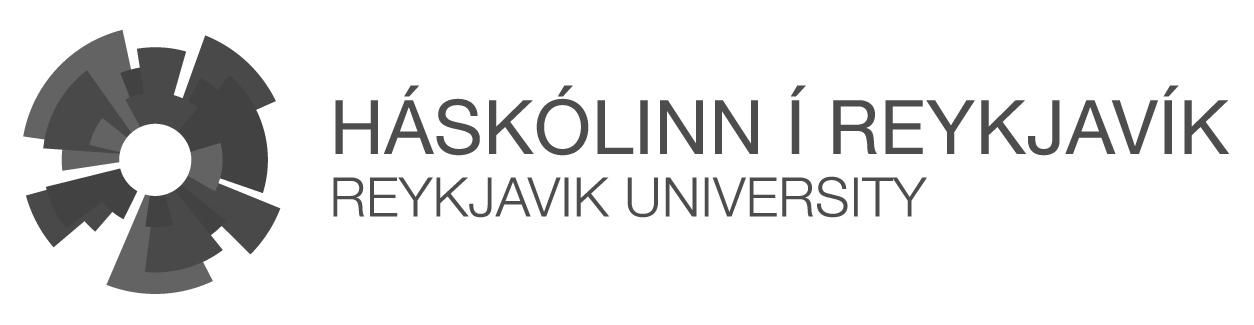
\includegraphics[width=5cm]{HR-Logo-bw} \\Artificial Intelligence\\ Lab 1 - Agents}
\author{Geir Matti Järvelä \and Þorgeir Auðunn Karlsson}
\lhead[lh-even]{T-622-ARTI - Artificial Intelligence}
\rhead[rh-even]{Geir Matti Järvelä (geirmj11@ru.is) \\ Þorgeir Auðunn Karlsson (thorgeirk11@ru.is)}

\begin{document}
\maketitle
\section{Heuristic function}
The heuristic we use is quite simple(if somewhat overly optimistic). We take the manhattan distance from the current point to all patches of dirt, 
ignoring obstacles. This gives us an extremely short path length, in fact a path that can only be achieved if there is only one node left, and it is on the 
starting point. This will never overestimate the cost, since even at the extreme case where we have two nodes on each side of the current position, 
the heuristic function will return a value of 4, while the actual path is 4 plus turns(see picture). 
Since the function will never overestimate the cost, it is admissible. \\ \\
\begin{tikzpicture}
\draw [very thick,black] (0,0) -- (0,3);
\draw [very thick,black] (1,0) -- (1,3);
\draw [very thick,black] (2,0) -- (2,3);
\draw [very thick,black] (3,0) -- (3,3);
\draw [very thick,black] (0,0) -- (3,0);
\draw [very thick,black] (0,1) -- (3,1);
\draw [very thick,black] (0,2) -- (3,2);
\draw [very thick,black] (0,3) -- (3,3);
\node at (1.5,0.5){\small{dirt}};
\node at (1.5,1.5){\small{robot}};
\node at (1.5,2.5){\small{dirt}};
\draw [->, very thick, black] (0.5,1.6) -- (0.5,2.4) node [left] at (0.5,2.2) {$1$};
\draw [->, very thick, black] (0.5,1.4) -- (0.5,0.6) node [left] at (0.5,0.8) {$1$};
\node [below=0.2cm, align=center,text width=16cm] at (4.5,0)
        {
           Figure 1: Heuristic value(on the left) is 1 + 1 = 2 while the real path value(on the right) is 1+2+1=4
        };
        
\draw [very thick,black] (6,0) -- (6,3);
\draw [very thick,black] (7,0) -- (7,3);
\draw [very thick,black] (8,0) -- (8,3);
\draw [very thick,black] (9,0) -- (9,3);
\draw [very thick,black] (6,0) -- (9,0);
\draw [very thick,black] (6,1) -- (9,1);
\draw [very thick,black] (6,2) -- (9,2);
\draw [very thick,black] (6,3) -- (9,3);
\node at (7.5,0.5){\small{dirt}};
\node at (7.5,1.5){\small{robot}};
\node at (7.5,2.5){\small{dirt}};
\draw [->, very thick, black] (8.7,1.6) -- (8.7,2.4) node [left] at (8.6,2.2) {$1$};
\draw [->, very thick, black] (6.3,2.4) -- (6.3,0.6) node [right] at (6.3,1.5) {$2$};        
\draw [->, very thick, black] (8.7,0.6) -- (8.7,1.4) node [left] at (8.6,0.8) {$1$};
\end{tikzpicture} 
\begin{lstlisting}[caption=The heuristic function]
public static int heuristic(WeightedState state){
    int returnValue = 0;
    for(Point p : state.dirt){
        int temp = ((p.x-state.curPos.x)*(p.x-state.curPos.x)
                   +(p.y-state.curPos.y)*(p.y-state.curPos.y));
        returnValue += temp;
    }
    return returnValue;
}
\end{lstlisting}
\section{Experiments}
\subsection{Results from experiments}
\subsubsection{vacuumcleaner\_obstacles\_1.gdl}
$\bullet$ {\bf Breadth First search time complexity: } 34.200.181 nanoseconds. \\
$\bullet$ {\bf Breadth First search resulting points: } 55 points. \\
$\bullet$ {\bf Depth First search time complexity: } 6985928 nanoseconds. \\
$\bullet$ {\bf Depth First search resulting points: } 23 points. \\
$\bullet$ {\bf Uniform search time complexity: } 140.882.722 nanoseconds.\\
$\bullet$ {\bf Uniform search resulting points: } 57 points.\\
$\bullet$ {\bf A* search time complexity: } \\ 
$\bullet$ {\bf A* search resulting points: }\\
\subsubsection{vacuumcleaner\_obstacles\_2.gdl}
$\bullet$ {\bf Breadth First search time complexity: } 17.670.281 nanoseconds. \\
$\bullet$ {\bf Breadth First search resulting points: } 56 points. \\
$\bullet$ {\bf Depth First search time complexity: } 6.493.739 nanoseconds. \\
$\bullet$ {\bf Depth First search resulting points: } 36 points. \\
$\bullet$ {\bf Uniform search time complexity: } 92.278.934 nanoseconds. \\
$\bullet$ {\bf Uniform search resulting points: } 56 points.\\
$\bullet$ {\bf A* search time complexity: } \\ 
$\bullet$ {\bf A* search resulting points: }\\
\subsubsection{vacuumcleaner\_obstacles\_3.gdl}
$\bullet$ {\bf Breadth First search time complexity: } 60.054.491.709 nanoseconds. \\
$\bullet$ {\bf Breadth First search resulting points: } 704 points. \\
$\bullet$ {\bf Depth First search time complexity: } 209082645 nanoseconds. \\
$\bullet$ {\bf Depth First search resulting points: } 0 points (here it found a solution taking more than the maximum 
number of allowed steps. \\
$\bullet$ {\bf Uniform search time complexity: } nanoseconds. \\
$\bullet$ {\bf Uniform search resulting points: } points. \\
$\bullet$ {\bf A* search time complexity: } \\ 
$\bullet$ {\bf A* search resulting points: }\\
\subsubsection{vacuumcleaner\_obstacles\_4.gdl}
$\bullet$ {\bf Breadth First search time complexity: } 25.422.995.901 nanoseconds. \\
$\bullet$ {\bf Breadth First search resulting points: } 790 points. \\
$\bullet$ {\bf Depth First search time complexity: } 171.459.937 nanoseconds.\\
$\bullet$ {\bf Depth First search resulting points: } 87 points.\\
$\bullet$ {\bf Uniform search time complexity: } nanoseconds. \\
$\bullet$ {\bf Uniform search resulting points: } points. \\
$\bullet$ {\bf A* search time complexity: } \\ 
$\bullet$ {\bf A* search resulting points: }\\
\subsubsection{vacuumcleaner\_obstacles\_5.gdl}
$\bullet$ {\bf Breadth First search time complexity: } 53.500.219.883 nanoseconds. \\
$\bullet$ {\bf Breadth First search resulting points: } 830 points. \\
$\bullet$ {\bf Depth First search time complexity: } 156.906.161 nanoseconds\\
$\bullet$ {\bf Depth First search resulting points: } 0 points (again, too many steps)\\
$\bullet$ {\bf Uniform search time complexity: } nanoseconds. \\
$\bullet$ {\bf Uniform search resulting points: } points. \\
$\bullet$ {\bf A* search time complexity: } \\ 
$\bullet$ {\bf A* search resulting points: }\\

\subsubsection{vacuumcleaner\_obstacles\_6.gdl}
$\bullet$ {\bf Breadth First search time complexity: } 8.834.495.039 nanoseconds.  \\
$\bullet$ {\bf Breadth First search resulting points: } 745 points. \\
$\bullet$ {\bf Depth First search time complexity: } 6.940.366.331 nanoseconds. \\
$\bullet$ {\bf Depth First search resulting points: } 773 points. \\
$\bullet$ {\bf Uniform search time complexity: } nanoseconds. \\
$\bullet$ {\bf Uniform search resulting points: } points. \\
$\bullet$ {\bf A* search time complexity: } \\ 
$\bullet$ {\bf A* search resulting points: }\\

\subsubsection{vacuumcleaner\_obstacles\_7.gdl}
$\bullet$ {\bf Breadth First search time complexity: } 512.934.332 nanoseconds.\\
$\bullet$ {\bf Breadth First search resulting points: } 710 points. \\
$\bullet$ {\bf Depth First search time complexity: } 167.453.066 nanoseconds. \\
$\bullet$ {\bf Depth First search resulting points: } 0 points (took 971 steps). \\
$\bullet$ {\bf Uniform search time complexity: } nanoseconds. \\
$\bullet$ {\bf Uniform search resulting points: } points. \\
$\bullet$ {\bf A* search time complexity: } \\ 
$\bullet$ {\bf A* search resulting points: }\\

\subsubsection{vacuumcleaner\_obstacles\_8.gdl}
$\bullet$ {\bf Breadth First search time complexity: } 1.185.210.774 nanoseconds.\\
$\bullet$ {\bf Breadth First search resulting points: } 685 points.\\
$\bullet$ {\bf Depth First search time complexity: } 165.483.396 nanoseconds. \\
$\bullet$ {\bf Depth First search resulting points: } 0 points(too many steps). \\
$\bullet$ {\bf Uniform search time complexity: } nanoseconds. \\
$\bullet$ {\bf Uniform search resulting points: } points. \\
$\bullet$ {\bf A* search time complexity: } \\ 
$\bullet$ {\bf A* search resulting points: }\\

\subsubsection{vacuumcleaner\_obstacles\_9.gdl}
$\bullet$ {\bf Breadth First search time complexity: } 4.006.193.735 nanoseconds. \\
$\bullet$ {\bf Breadth First search resulting points: } 690 points. \\
$\bullet$ {\bf Depth First search time complexity: } 194.238.702 nanoseconds.\\
$\bullet$ {\bf Depth First search resulting points: } 0 points(too many moves).\\
$\bullet$ {\bf Uniform search time complexity: } nanoseconds. \\
$\bullet$ {\bf Uniform search resulting points: } points. \\
$\bullet$ {\bf A* search time complexity: } \\ 
$\bullet$ {\bf A* search resulting points: }\\

\subsubsection{vacuumcleaner\_obstacles\_10.gdl}
$\bullet$ {\bf Breadth First search time complexity: } 16.021.984.525 nanoseconds. \\
$\bullet$ {\bf Breadth First search resulting points: } 705 points. \\
$\bullet$ {\bf Depth First search time complexity: } 184.201.863 nanoseconds.\\
$\bullet$ {\bf Depth First search resulting points: } 0 points(once more the path was too long). \\
$\bullet$ {\bf Uniform search time complexity: } nanoseconds. \\
$\bullet$ {\bf Uniform search resulting points: } points. \\
$\bullet$ {\bf A* search time complexity: } \\ 
$\bullet$ {\bf A* search resulting points: }\\

\subsection{Conclusions}
Not surprizingly Depth first search is probably the worst of the bunch. It gets the job done fast, i.e. it finds 'a' path fast, but 
picks a highly random and usually stupid path. Only once did it beat the score of 
the BFS, but since BFS doesn't take into account turning costs, this is bound to happen every once in a while.\\

Breadth first search was a surprize here, when given enough time (and not even a lot more), it gave very good results, even if it didn't take the cost 
of turning into account. A clear winner for simplicity. Relative to the other search methods it takes a lot of time, but in small cases it is quite good enough. \\

Uniform search and A* Search were surprizingly slow, but this is mainly due to an implementation error in Java. We used priorityQueue to implement the searches
and found out just before handing in that remove operations in priority queue are incredibly slow. Sadly this slows down the total calculations, but would have 
been easy to avoid if we would have known beforehand about this problem.

A* Search
\end{document}
